% fdps_sc15.tex
% paper about FDPS for SC 15
% Author: A. Tanikawa
% 1 March 2015

\documentclass[dvipdfmx]{acm_proc_article-sp}
%%%%%%%%%%%%%%%%%%%%%%%%%%%%%%%%%%%%%%%%%%%%%%%%%%%%%%%%%%%%%%%%
\usepackage{listings}
\usepackage{color}
\newcommand{\myvec}[1]{\vec{#1}}
\newcommand{\redtext}[1]{\textcolor{red}{#1}}
\newcommand{\araa}{Annual Review of Astronomy and Astrophysics}
\newcommand{\icarus}{Icarus}
\newcommand{\mnras}{Monthly Notices of the Royal Astronomical Society}
\newcommand{\apj}{Astrophysical Journal}
\newcommand{\pasa}{Publications of the Astronomical Society of Australia}
\newcommand{\pasj}{Publications of the Astronomical Society of Japan}
\newcommand{\aap}{Astronomy and Astrophysics}
\newcommand{\nat}{Nature}
%%%%%%%%%%%%%%%%%%%%%%%%%%%%%%%%%%%%%%%%%%%%%%%%%%%%%%%%%%%%%%%%

\begin{document}

\title{Extreme-scale, High-performance Parallel Computing at Your
  Fingertip --- A Framework for Particle-based Simulations, FDPS}


%\subtitle{}

\numberofauthors{5}

\author{
  \alignauthor
  Masaki Iwasawa \\
  \affaddr{RIKEN Advanced Institute for Computational Science} \\
  \affaddr{7--1--26, Minatojima-minami-machi, Chuo-ku, Kobe, Hyogo, Japan} \\
  \email{masaki.iwasawa@riken.jp}
  %
  \alignauthor
  Ataru Tanikawa \\
  \affaddr{RIKEN Advanced Institute for Computational Science} \\
  \affaddr{7--1--26, Minatojima-minami-machi, Chuo-ku, Kobe, Hyogo, Japan} \\
  \email{ataru.tanikawa@riken.jp}
  %
  \alignauthor
  Natsuki Hosono \\
  \affaddr{RIKEN Advanced Institute for Computational Science} \\
  \affaddr{7--1--26, Minatojima-minami-machi, Chuo-ku, Kobe, Hyogo, Japan} \\
  \email{natsuki.hosono@riken.jp}
  \and
  %
  \alignauthor
  Keigo Nitadori \\
  \affaddr{RIKEN Advanced Institute for Computational Science} \\
  \affaddr{7--1--26, Minatojima-minami-machi, Chuo-ku, Kobe, Hyogo, Japan} \\
  \email{keigo@riken.jp}
  %
  \alignauthor
  Takayuki Muranushi \\
  \affaddr{RIKEN Advanced Institute for Computational Science} \\
  \affaddr{7--1--26, Minatojima-minami-machi, Chuo-ku, Kobe, Hyogo, Japan} \\
  \email{takayuki.muranushi@riken.jp}
  %
  \alignauthor
  Junichiro Makino \\
  \affaddr{RIKEN Advanced Institute for Computational Science} \\
  \affaddr{7--1--26, Minatojima-minami-machi, Chuo-ku, Kobe, Hyogo, Japan} \\
  \email{jmakino@riken.jp}
}

\maketitle

%% % Justification We report the performance of applications
%% developped using FDPS, a framework for developing particle
%% simulators. FDPS provides a class template library for the
%% parallelization procedures for parallelized particle-simulation
%% code. Using FDPS, researchers can develop highly-scalable, highly
%% efficient simulations programs in a very short time. We believe
%% this is important contribution to HPC.



\begin{abstract}

  As an entry to the ACM Gordon Bell Prize for year 2015, we report
  the concept, implementation, and performance of FDPS (Framework for
  developing particle simulators).  The basic idea of FDPS is to
  separate the program code for complex parallelization such as domain
  decomposition, redistribution of particles, and exchange of particle
  information for interaction calculation between nodes, from actual
  interaction calculation and orbital integration. The former part is
  taken care by FDPS. Users of FDPS write the
  latter part. Using FDPS, a program for gravitational $N$-body
  simulation can be written in less than 120 lines,
  and yet, it will run on large machines like K computer or Cray XC30
  with near-ideal scalability. Also, very high efficiency such as
  $\sim 50$\% of the theoretical peak can be achieved. We report the
  performance of two applications. Both application achieved
  near-ideal weak-scaling performance on two architectures, with very
  high execution efficiency.


\end{abstract}

\category{D.1.3}{Software}{PROGRAMMING TECHNIQUES}[Concurrent
  Programming]
%%
\category{I.6.7}{Computing Methodologies}{SIMULATION AND
  MODELING}[Simulation Support Systems]
%%
\category{J.2}{Computer Applications}{PHYSICAL SCIENCES AND
  ENGINEERING}[Astronomy]
%%
\category{J.2}{Computer Applications}{PHYSICAL SCIENCES AND
  ENGINEERING}[Earth and atmospheric sciences]
%%
\terms{Algorithm, Performance}
%%
\keywords{Framework for implementing parallel codes, high-performance
  computing, particle simulation}

\section{Introduction}

Development of an application program which achieves high efficiency on
modern HPC platforms has become a multi-person, multi-year project.
In Japan, while K computer was being developed, ``Grand Challenge''
program was underway, of which the goal was to develop
high-performance, highly-parallelized applications optimized for K
computer. Also, for the so-called ``post-K'' project, nine ``priority
fields'' and also nine ``target applications'' have been
selected. These target applications are used for the co-design of
software and hardware.

The existence and history of the Gordon Bell Prize itself indicate how
difficult it is to develop high-performance parallel application
programs. This year's announcement for the Gordon Bell Prize states:

\begin{quote}
   The Gordon Bell Prize is awarded each year to recognize outstanding
   achievement in high-performance computing. The purpose of the award
   is to track the progress over time of parallel computing, with
   particular emphasis on rewarding innovation in applying
   high-performance computing to applications in science, engineering,
   and large-scale data analytics. Prizes may be awarded for peak
   performance or special achievements in scalability and
   time-to-solution on important science and engineering problems.
\end{quote}

Thus, it is clear that innovation is considered to be necessary to
advance parallel computing, and that scalability and time-to-solution
are considered important. In fact, if we look back the history of the
Gordon Bell Prize, we can clearly see that many awards have been given
essentially to the demonstration that the newest and fastest machine
at that time can be actually used for some real applications with
reasonable efficiency. 

To achieve a reasonable efficiency has been becoming more and more
difficult in the entire history of the Gordon Bell Prize, and is
expected  to become even more so in the foreseeable future. There are
many factors which make the efficient use of modern HPC platforms
increasingly more difficult. They include:

\begin{enumerate}

  \item The increase in the number of processors. In 1993, high-end
    Cray T3D or TMC CM-5 had 1024 processors. In 2011, K computer had
    88,128 processors.
  \item The increase in the number of cores per processor. The DEC
    Alpha 21064 processor used in Cray T3D had just one core. K computer
    had 8 cores. Present-day Xeon-based systems have 20-36 cores per
    node, and Xeon Phi has $>60$ cores.
  \item The increase in the number of floating point units per core.
    The DEC     Alpha 21064 processor had one. One core of the K
    computer had four, and Haswell Xeon has eight. Cores with 16
    floating-point units are expected to appear in several years.
  \item The decrease in the memory bandwidth relative to the
    floating-point performance. Cray T3D had the B/F or around 2.5.
    K computer 0.35, and Xeon Phi 0.28. The relative increase of the
    memory latency adds to the difficulty. 
  \item The decrease in the network bandwidth relative to the floating
    point performance. T3D had a 3D torus with 300MB/s links, with
    nominal one-direction network B/F of 2. For K computer, this
    number is 0.078125.
\end{enumerate}

The only factor which helped to make the use of large machines easier
is the increase of the problem size that can be solved. The fact that
problem size increased implies that the relative cost of
interprocessor communication can be reduced, if clever
spatial decomposition is used.

In the late 80's and early 90's, parallel languages such as CM-Fortran
(or HPF) could be used to develop high-performance applications. This
is simply because the machines then had sufficient memory bandwidth
and network bandwidth. At present, however, we do not have such
luxury.  We cannot use vectorizing compilers to make use of multiple
cores and SIMD units either, because of the large latency associated
with fork/join and low memory bandwidth. We need to carefully design
our program so that it can make use of
multiple cores, SIMD units and cache hierarchy. Thus a program which
does just a simple calculation becomes very complicated.

Even though parallel computing has been an active area of
research in the last two decades, to use high-end machines has become
increasingly more difficult, and the full configuration of largest
machines are applied  only to small number of ``really big''
calculations, simply because they cannot solve small problems
fast. Even for such big problems, in many cases  the achieved efficiency
is surprisingly low, around 10\% of the theoretical peak or less.

This problem of the large-scale parallel computing today is well
recognized by researchers, and that must be the reason why the
statement for Gordon Bell Prize highlights scalability and
time-to-solution. Concerning time-to-solution, in many cases the
actual time spent by the computer is no longer the most important
factor, and the time and total amount of human resources we need to
develop programs has become most critical. In order to study a new
problem using large-scale simulations, in many cases we need to modify
existing simulation programs, or to develop a new one.  As we stated
earlier, the latter would take many years, while the former is very
difficult or impossible for researchers other than the developer of
that program. Moreover, when a big machine is replaced by a new one,
application programs require modifications to achieve similar level of
efficiency, since the new machine probably has more cores, wider SIMD
units, less memory and network bandwidth. Thus, just to keep
application programs up-to-date is becoming a big enterprise.

For the last several years, we have been working on what we believe
will help resolving this difficulty, at least for a limited class of
applications: particle-based simulations.

Particle-based simulations have been widely used in the field of
computational science, and they are becoming more and more popular. In
particle-based simulations, a system under study is regarded as a
collection of mutually-interacting particles, and its evolution is
described by the evolution (in many cases, motion) of individual
particles. Examples of particle-based simulations include
gravitational $N$-body simulation, molecular dynamics simulation,
granular dynamics simulation, and element-free simulation of fluid
dynamics or structural analysis.

Most of particle-based simulations share one common characteristics:
the calculation cost of particle-particle interaction is
dominant. Thus, in order to achieve high efficiency, it is critical to
optimize the interaction calculation, but optimization of the rest of
the code is not so critical. Of course, when we try to run our code on
a 100k-node, 1M-core machine, the rest of the code should be
parallelized over 100k nodes with very good load balance, but very
high efficiency is not a high priority for calculations other than the
interaction calculation.

In order to parallelize a program for particle-based simulation, we
need to implement (a) domain decomposition, (b) exchange of particles
according to the domain decomposition, (c) exchange of the information
necessary to calculate the interaction between particles in different
domain. Just to implement these procedures correctly is difficult,
and to achieve high scalability is even more difficult.

Of course, it is not impossible to realize such a highly efficient
implementation for a specific problem. For example, the gravitational
$N$-body problem has been well studied, and several impressive
achievements have been reported {\cite{confscWarrenSBGSW97,
    2004PASJ...56..521M, 2005Natur.435..629S,
    Hamada:2009:THN:1654059.1654123, Hamada:2010:TAN:1884643.1884644,
    ishiyama:gordonbell, Bedorf:2014:PGT:2683593.2683600}}.  However,
when researchers in other fields want to achieve similar performance
on their own particle-based simulations, there has been no easy way to
reuse efficient codes, simply because they were not designed to be
applied to different problems.

We have designed and developed FDPS, (Framework for Developing
Particle Simulator)\footnote{https://github.com/FDPS/FDPS}, to solve
this problem. FDPS provides the codes to perform the above procedures
(a) to (c), for particle-based simulation codes with arbitrary
definition of particles and interaction between particles.  In
addition, FDPS supplies an efficient tree-based calculation routine
for both long-range and short-range interactions. Thus, researchers
who use FDPS can concentrate on the description of the physical
process and numerical schemes, letting FDPS does the complicated
parallelization.

In this paper, we briefly overview the structure and implementation of
FDPS, and then report the performance of two applications
(astrophysical $N$-body simulation and SPH simulation) developed using
FDPS on two different architectures: K computer and Cray XC30 (with
Haswell processors) of National Astronomical Observatory of Japan.

For all of four combinations of applications and architectures, we
observed very good scalability, even though application-specific,
user-developed part of the program contains no code for
parallelization. In order to achieve high execution efficiency, it is
sufficient to provide the interaction kernel optimized to either
generic SIMD execution units or more specialized kernel for a given
architecture. 

In section 2, we overview the design concept and the structure of
FDPS. Since the basic principle has been described elsewhere
{\cite{2015iwasawa}}, here we just summarize the design
concept. In section 3, we discuss some of the technical details
important to achieve high scalability. In section 4, we present the
measured performance of two applications developed using FDPS on two
platforms. Section 5 summarizes the paper.

\section{Design concept of FDPS}

\label{sec:designconcept}


In this section, we describe the design concept of FDPS.  The goal of
FDPS is to let the users develop their own programs in short time, and
yet enjoy high scalability and high performance. One possible way to
achieve this goal is to let the users write their codes using some
specially-designed language (domain-specific language, or DSL), and
develop a translator which generate from the description of the
problem in DSL into C or Fortran. There are many researchers working
in this direction, but most of them focus on grid-based
calculation. For FDPS, we chose a different approach. The users of
FDPS write their programs using standard high-level languages, with
several function calls to FDPS library. When compiled using MPI
compiler, FDPS library functions resulted in a parallel code which use
MPI functions. If compiled using compilers without MPI support, a
non-MPI execution code is generated. The same is true for the use of
OpenMP.

Conceptually, an application program which uses FDPS library works as
follows.

\begin{enumerate}

  \item It reads in a parameter file (or parses command line options)
    to obtain runtime parameters
  \item It reads in the initial condition from file(s), or generates
    it.
  \item It repeats the following steps (4 to 6) until it reaches the end of
    simulation (or near the end of CPU time limit).
  \item It calculates the interaction between particles.
  \item It performs the integration of trajectories of particles.
  \item When necessary, it performs the on-the-fly analysis of the
    system and generates output.
\end{enumerate}

Steps 1 and 2 are not taken care by FDPS. Thus, for these steps, the
user program should describe how it operates in environment with MPI,
as well as without MPI.  In order to simplify this part, we provide
wrapper functions for some of MPI functions, so that programs written
using those wrapper functions can be compiled and run in environment
without MPI support. For example, in order to read in a parameter file
in an MPI program, usually we write a code in which the process with
rank 0 reads in the parameters and then broadcasts them to other
nodes. If a user uses {\tt MPI\_Comm\_rank} and 
 {\tt MPI\_Bcast} to implement this part, the
resulted source code requires MPI library. To avoid this complicacy,
we provide wrapper functions within FDPS, so that user programs which
uses these wrappers can be compiled in environments without MPI
support. The same is true for the file I/O and analysis of the result.
It is also possible to write the application program which explicitly
use MPI. In this case, it should be compiled using compilers with MPI
support, even for single-node execution. Users of FDPS can select the
approach more convenient for them.

At the end of step 2, the user program has the initial condition
set, in an array of particle class. This class itself is defined in
the user program. In the case of an MPI environment, at this point, all
processes must share the input parameters, but there is no
restrictions on the way they have particles, except that there should
not be any overlap. It is okay that rank 0 process has all
particles. It is also okay that each process has some number of
particles, and at this moment it is not necessary that particles are
partitioned into subdomains.

Step 4 is implemented using FDPS library functions, in the following
substeps.

\begin{description}

  \item{a)} decompose the computational domain.
  \item{b)} exchange particles so that all particles belong to
    the correct process.
   \item{c)} collect the information of particles
     in other processes necessary for the interaction calculation.
   \item{d)} calculate the interaction.

\end{description}
Note that particles are actually exchanged between processes in
substep (b). Therefore, the user program should not assume that a
particle that is  initially in its domain will remain there. Particles 
move from one process to another, depending on the geometry of domain
decomposition and their positions. 

Step 5 is implemented entirely in the user program.  Many integration
schemes need to calculate the interaction more than once per
timestep. When such schemes are used, it is necessary to call FDPS
functions to calculate interactions multiple times. In this case, only
substeps (c) and (d) should be done, since particles should not move
from one process to another during one timestep.

Step 6 is also implemented entirely in the user program.
For the analysis and diagnostics,  a quantity which requires global
reduction operations are sometimes necessary. Therefore we provide
wrapper functions for reduction functions in MPI, so that a user
program  can be compiled without using MPI. 

Since steps 5 and 6 are implemented entirely in the user program, any
operation can be done in these steps. Examples of operations include
the addition of external field, implementation of physical collisions
between particles, implementation of physical processes other than the
particle-particle interactions (for example supernova explosion in
simulations of star clusters or galaxy in the case of astrophysical
simulations).

For steps 1,2,5 and 6, the users of FDPS write their programs
essentially in the same way  as  they write programs
parallelized using MPI. However, communications used in these steps
are generally simple.  For step 4, in which all the complex operations
for parallelization and optimization is hidden, the only thing the
users of FDPS need to do is to write the function to calculate
interaction between particles, and write the calls to necessary FDPS
functions.  As we stated earlier, in order to achieve high efficiency
the function to calculate interactions should take advantage of SIMD
units available. It is not necessary to use multiple cores in this
function, since multithreading is taken care by FDPS.

Thus, the length of the user code developed using FDPS is short, since
all complex operations for parallelization are done in FDPS function
calls in step 4. This also means that the development process of
application program is much simpler than that of usual large-scale
parallel program developed using MPI, resulting in much shorter
development time.

\section{Implementation details}

The basic structure of FDPS is described elsewhere
\cite{2015iwasawa}. Here, we first briefly go through the
general structure of FDPS and algorithms used in it, and then discuss
performance- and flexibility-related issues.

\subsection{General structure  and algorithms used}

The main functionalities of FDPS are, as described in the previous
section, (a) domain decomposition, (b) exchange of particles according
to the domain decomposition, (c) exchange of the information necessary
to calculate the interaction between particles in different domain and
(d) actual calculation of the interaction. In the following, we
briefly visit these functions.

First of all, in FDPS these are implemented as class template 
libraries in C++. We decided to use the class template in order to
achieve the flexibility without sacrificing the performance. FDPS
functions should operate on user-defined particles. This means that
FDPS functions are ``abstractions'' of actual functions for a given
particle class. The class template of C++ language offers convenient
and efficient way to realize such abstractions. FDPS library functions
are provided as source programs, or header files for user programs. 
They are called with the particle class as template
parameter. When the user program is compiled, the class template is
``instantiated'' or ``specialized'' with the user-defined class, and
then compiled.  Thus, there is no overhead associated with the
interface between the FDPS library functions and in the particle
class. This use of class template is very important to achieve high
performance.

For domain decomposition, we used the multisection method
\cite{2004PASJ...56..521M} with the so-called sampling
method \cite{Blackston:1997:HPE:509593.509597}. The
multisection method is a generalization of ORB (Orthogonal Recursive
Bisection). In ORB, as its name suggest, bisection is applied to each
coordinate axis recursively. In multisection method, division in one
coordinate is not to two domains but to an arbitrary number of
domains. Since one dimension can be divided to more than two sections,
it is not necessary to apply divisions many times. So we apply
divisions only once to each coordinate axis. A practical advantage of
this method is that the number of processors is not limited to powers
of two.

In the sampling method, first each process performs random sampling of
particles under it, and sends them to the process with rank 0
(``root'' process hereafter). Then the root process calculates the
division so that sample particles are equally divided over all
processes, and broadcasts the geometry of domains to all other
processes. In order to achieve good load balance, sampling frequency
should be changed according to the calculation cost per particle
\cite{ishiyama:greem}.

To achieve the exchange of particles,
each  process then sends out particles which are outside its domain,
to the correct destination process. This is easy to implement since 
each process has the complete information of domain decomposition. 

The interaction calculation is performed in the following steps.
First, each process constructs the octree structure of particles. This
tree structure is used to determine, for each of other processes, what
information should be sent. In the case of long-range interactions,
particles and superparticles (corresponding to tree nodes) are
sent. In the case of short-range interactions, particles are sent.

After each process receives all the information necessary, it
reconstruct the tree structure. This tree structure is now used to
calculate interaction. The tree is traversed for a group of particles,
and ``interaction list'' is created for this group of particles
\cite{1990JCoPh..87..161B}. Finally, the list of particles
in the group and particles in the interaction list are both passed to
the user-supplied interaction calculation function, in which the
actual force calculation is performed.


\subsection{Performance-related issues}

Here, we discuss some of the performance-related issues, which turned
out to be important when very large number of processors are used. 

The sampling method works fine, if the number of particles per process
is significantly larger than the number of process. This is, however,
not the case for runs with a large number of nodes.  For example, K
computer has more than 80,000 nodes, and in this paper we report the
result of runs with almost all nodes. Even with the number of
particles per process same as the number of nodes, the total number of
particles becomes 6.4 billion, and we do want to run simulations with
smaller number of particles.

When the number of particles per process is not much larger than the
number of processes, the total number of sample particles which the
root process need to handle exceeds the number of particles per
process itself, and thus calculation time of domain decomposition in the
root process becomes visible. In order to reduce the calculation time,
we implemented two-stage hierarchical sampling, in which processes
with index $(i,0,0)$, in other words, the root processes in each of y-z
plane, collect samples, and then create subsamples to be sent to the
root process. After the root process determines the division in
x-direction, 
processes with index $(i,0,0)$ exchange the sample particles and then
construct the divisions in y-z planes. It is also possible to
implement three-stage sampling,  but even for the full-node runs on K
computer we found the two-stage sampling is sufficient.

For exchange of particles and also for the exchange of data necessary
for interaction calculation, we use {\tt
    MPI\_Alltoall} to exchange the length of the data and
{\tt MPI\_Alltoallv} to actually
exchange the data. At least on K computer, we found that the
performance of vendor-provided {\tt
    MPI\_Alltoall(v)} is not optimal for short messages. We
implemented a hand-crafted version in which the messages sent to the
same relay points are combined in order to reduce the total number of
messages.

\subsection{Flexibility-related issues}

Here, we discuss some of the minor (but practically important)
aspects of particle-based simulations and how they are handled in
FDPS. Those are the followings
\begin{itemize}

  \item Multiple species of particles
  \item Boundary conditions
  \item particle-particle interactions which cannot be described as
    the summation of two-body interactions
  \item The use of heterogeneous multiprocessors such as GPGPUs.
\end{itemize}

In some of particle-based simulations, we want to handle particles of
different types, which interact through different interaction
functions. For example, when we simulate a galaxy, we need particles
which represent stars or dark matter, and particles which represents
interstellar gas. The former particles interact with other particles
only through gravity, while the latter through both gravity and
hydrodynamics interactions. Therefore, FDPS is designed to handle
multiple types particles and multiple types of interactions. It is
possible that particles of different types interact through one
interaction function (for example gravity). It is also possible that
particles of one type interact through multiple interactions (for
example gravity and hydrodynamics). 

For the boundary condition, currently we provide the support for the
open boundary condition and periodic boundary (can be specified for
each of coordinate axes separately). For the long-range, $1/r$
potential, currently we offer a library for a low-order Particle-Mesh
scheme \cite{hockney1988computer, 1995ApJS...98..355X,
    2000ApJS..128..561B, 2002JApA...23..185B, 2004NewA....9..111D,
    springel:gadget2, 2005PASJ...57..849Y, ishiyama:greem,
    ishiyama:gordonbell}, which can be used in combination with
particle-particle interaction calculation with long-range cutoff. We
plan to provide higher-order, high-accuracy libraries in the future
release.

In some of particle-based calculations, we need to calculate
interparticle forces which cannot be described as the summation of
two-body interactions. For example, in molecular dynamics simulations
of complex molecules such as proteins, ``bonding'' forces of various
types need to be evaluated. Of course, this evaluation can be
implemented in the user code for step 5 described in the previous
section. However, particles participating in one bonding interaction
might exist in different processes. Even when all particles
participating in one bonding interaction are in the same process, the
application program need to find out, for each particle, what bonding
force should be evaluated with which particles. This can be done, but
currently requires rather complex programming.  It is probably
worthwhile to provide the FDPS library to evaluate bonding
interactions. We are studying the design of the API.

Many of HPC platforms now have heterogeneous architectures, such as
the combination of general-purpose CPUs and GPGPUs. With the current
design of FDPS, it is possible to use GPUs for the interaction
calculation, by writing the interaction calculation function using
CUDA or OpenCL. However, the performance achieved
will not be very good, since the degree of parallelism available in
the single call for the interaction function is not very large. We can
increase the parallelism by extending the interface of the interaction
calculation function, so that it is called for multiple pairs of
particles which exert the interactions and particles which receive the
force, in the same way as used in GPU implementation of Barnes-Hut
tree algorithm {\cite{hamada2009novel,
    Hamada:2009:THN:1654059.1654123, Hamada:2010:TAN:1884643.1884644,
    Bedorf:2014:PGT:2683593.2683600}}. We plan to include this
extended interface to future release.


\section{Measured performance}


In this section, we report
the measured
performance of two applications developed using FDPS on two
platforms. First, in  section \ref{sect:applications},
we describe the applications. In section
\ref{sect:userprograms}, we show the size of the source programs, and
in section \ref{sect:achievedperformance} achieved performance.



\subsection{Applications}
\label{sect:applications}

We report the performance of two applications: the gravitational
$N$-body simulation and the astrophysical fluid simulation with self
gravity implemented with SPH. For performance measurement, we used two
systems. One is K computer, and the other is Cray XC30 of CfCA,
National Astronomical Observatory of Japan. K computer consists of
82,944 Fujitsu SPARC64 VIIIfx processor, each with
eight cores. The theoretical peak performance of one core is 16
Gflops, for both of single- and double-precision operations. Cray XC30
of CfCA consists of 1060 nodes, or 2120 Intel Xeon E5-2690v3 processor
(12 cores, 2.6GHz). The theoretical peak performance of one core is
83.2 and 41.6 Gflops for single- and double-precision operations,
respectively.  For the gravitational $N$-body simulation, we were able
to use up to about 80k nodes of K computer. On Cray XC30, the maximum
number of cores we could use was 2064.

The equation of motion for the gravitational $N$-body simulation is
given by
\begin{equation}
  \mathbf{a}_i = \sum_{j\ne i} -G m_j\frac{\mathbf{r}_i-\mathbf{r}_j}
  {[(\mathbf{r}_i-\mathbf{r}_j)^2 + \epsilon^2 ]^{3/2}},
\end{equation}  
where $  \mathbf{a}_i$, $m_i$, $\mathbf{r}$ are acceleration,
mass, and position of particle $i$, $G$ is the gravitational constant
and $\epsilon$ is the softening parameter used to avoid the divergence
of the mutual force in the limit of $\mathbf{r}_i-\mathbf{r}_j
\rightarrow 0$.

We use the Barnes-Hut tree algorithm {\cite{1986Natur.324..446B}}
implemented in FDPS for the gravitational force calculation. Multipole
expansion up to quadrupole is used, and the opening angle for treewalk
is $0.4$.  We measured the performance for two test problems. One is
the evolution of a self-consistent galaxy model consisting of a
central bulge, stellar disk and dark matter halo. Another is a simple,
spherically symmetric Plummer model in the dynamical equilibrium. For
both tests, we measured the weak-scale performance, with the number of
particles per core fixed to 256k on K computer and on Cray XC30.

For the SPH simulation with self-gravity, We adopt the standard SPH
scheme \cite{1992ARA&A..30..543M, 2009NewAR..53...78R,
  2010ARA&A..48..391S} for the hydro part. Artificial viscosity
\cite{1997JCoPh.136..298M} with the standard Balsara switch
\cite{1995JCoPh.121..357B} is used to capture shocks.
We used the variable kernel length. The average number of particles
within the neighbor sphere of one particle is about 250.

We consider the simulation of the Giant Impact (GI).  The Giant Impact
scenario \cite{1975Icar...24..504H, 1976LPI.....7..120C} is at present
the most widely accepted scenario for the formation of the Moon.  In
the GI scenario, at the final stage of the formation of the Earth, a
Mars-sized object (hereafter, the impactor) collided with the
proto-Earth (hereafter, the target). The collision scattered a large
amount of debris, which first formed the debris disk and eventually
the Moon. Many researchers have performed simulations of GI, using the
SPH method.  \cite{1986Icar...66..515B, 2013Icar..222..200C,
  2014NatGe...7..564A}.  However, recent comparison with the grid code
indicated that the agreement is not so good
{\cite{2006ApJ...638.1180W, 2013Icar..222..200C}}. Moreover,
it has been pointed out that the standard SPH scheme used on all of GI
simulations has difficulty in handling the contact discontinuity
{\cite{2013MNRAS.428.2840H, 2013ApJ...768...44S,
    2013PASJ...65..108H, 2014hosono}}. Thus, it is very important to
perform high-resolution, high-accuracy calculation of GI with improved
numerical schemes and test the convergence. Unfortunately, the largest
calculation for which the scientific result has been reported used
only 1M particles {\cite{2013Icar..222..200C}}.  The largest
number of particles used for GI simulations is 100 million
\cite{2014LPI....45.2703T}, but no scientific results were given.
Here, we investigated the possibility of large calculations.  We adopt
equation of state of granite \cite{1986Icar...66..515B} for the
particles. The initial conditions, such as the orbital parameters of
the two objects, are the same as those in
\cite{1986Icar...66..515B}. In this paper, we report the weak scaling
performance with about $35000$ and $45000$ particles per core on K
computer and Cray XC30, respectively. For the largest
calculation, we used $1.0$ billion particles and 32768 cores.
Figure \ref{fig:viewGI} shows the density maps from one run with 9.9
million particles. 

\begin{figure}
  \begin{center}
    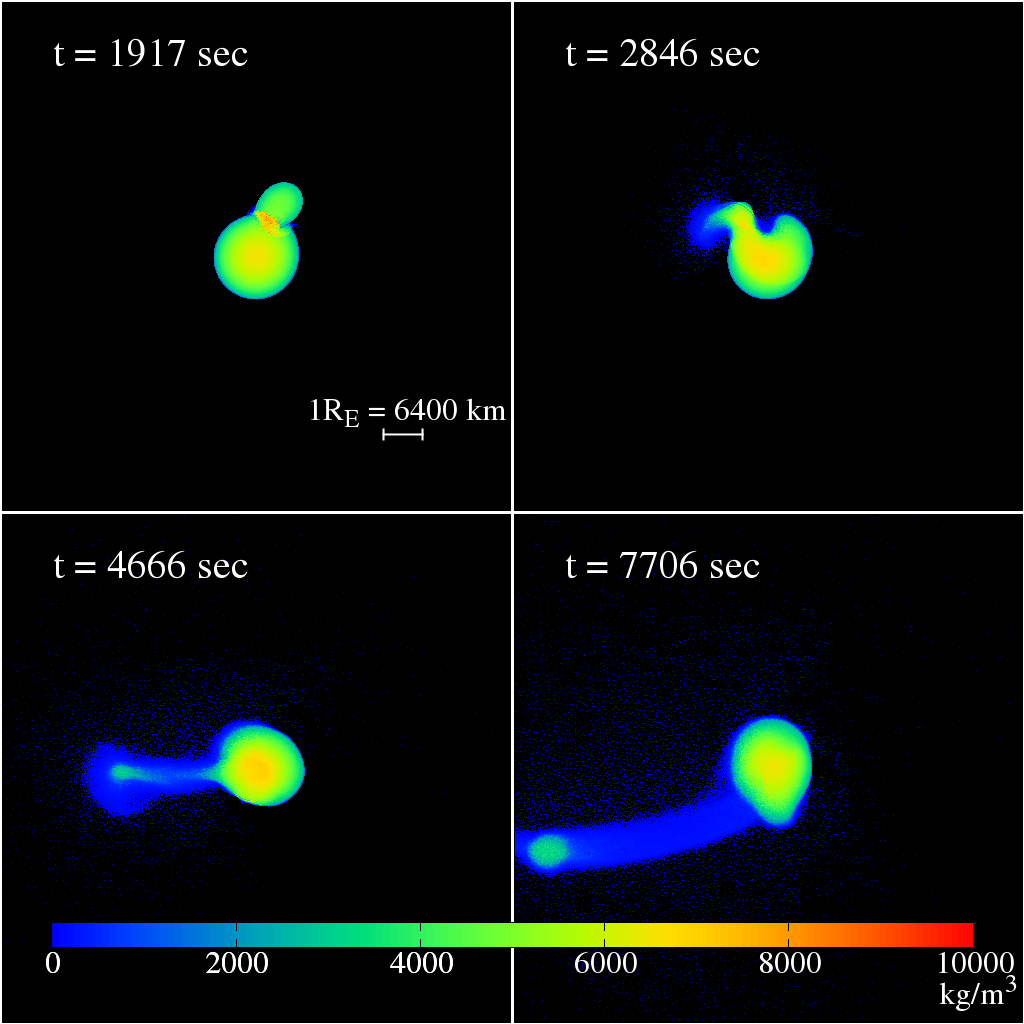
\includegraphics[width=8cm,bb=0 0 1024 1024]{gb.png}
  \end{center}
  \caption{Density maps of at the orbital plane for the run with
  $9.9$ million particles at four different epochs.
  }
  \label{fig:viewGI}
\end{figure}

\subsection{Size of user programs}
\label{sect:userprograms}

Before discussing the performance, 
here we show the size of the user
programs, in terms of the number of lines of source program.

In table \ref{tab:applicationsize} the sizes of applications in terms
of the number of lines of the source code are shown.

\begin{table}
  \begin{center}
  \caption{Size of the application programs}
  \label{tab:applicationsize}
  \begin{tabular}{lcc}
    \hline
      & $N$-body & SPH\\
    \hline
    Total & 801 & 1298 \\
    Particle definition &  51 & 226 \\
    Interaction Functions &  437 & 570 \\
    Initial setup and I/O &  128 & 96 \\
    Main integration loop &  12 & 49 \\
    Miscellanies & 173 & 357\\
\hline    
  \end{tabular}
  \end{center}
\end{table}

We can see that both programs are pretty compact, with total lines of
code less than 1,300. In the case of the $N$-body code, the number of
lines for functions to calculate two-body force is pretty large. This
is simply because optimization for the SIMD unit resulted in a rather
length code. Listing \ref{code:simpleforce} shows a simple code for
gravitational interaction calculation. This code can be actually used,
but performance would be not so good, since most of the compilers
available today do not generate very efficient assembly code from this
description.

\begin{lstlisting}[label=code:simpleforce,numbers=left,numbersep=5pt,frame=single,basicstyle=\ttfamily,caption=A sample code of $N$-body simulation]
template <class TPJ>
struct CalcGrav{
  void operator () (const Nbody * ip,
                    const S32 ni,
                    const TPJ * jp,
                    const S32 nj,
                    Nbody * force) {
    for(S32 i=0; i<ni; i++){
      F64vec xi  = ip[i].pos;
      F64    ep2 = ip[i].eps * ip[i].eps;
      F64vec ai = 0.0;
      for(S32 j=0; j<nj;j++){
        F64vec xj = jp[j].pos;
        F64vec dr = xi - xj;
        F64 mj  = jp[j].mass;
        F64 dr2 = dr * dr + ep2;
        F64 dri = 1.0 / sqrt(dr2);                
        ai -= (dri * dri * dri * mj) * dr;
      }
      force[i].acc += ai;
    }
  }
};
\end{lstlisting}

\begin{lstlisting}[label=code:tunedforce,numbers=left,numbersep=5pt,frame=single,basicstyle=\ttfamily,caption=A highly optimized force function for $N$-body simulation]
__attribute__ ((always_inline))
void inline_kernel_epj(const v2r8 eps2,
                       const v2r8 jp_xy,
		       const v2r8 jp_zm,
		       const v2r8 xi,
		       const v2r8 yi,
		       const v2r8 zi,
		       v2r8 &ax,
		       v2r8 &ay,
		       v2r8 &az,
		       v2r8 &pot){
  const v2r8_bcl xj(jp_xy);
  const v2r8_bch yj(jp_xy);
  const v2r8_bcl zj(jp_zm);
  const v2r8_bch mj(jp_zm);
  const v2r8 dx = xj - xi;
  const v2r8 dy = yj - yi;
  const v2r8 dz = zj - zi;
  const v2r8 r2   = ((eps2 + dx*dx)
                      + dy*dy) + dz*dz;
  const v2r8 ri1  = r2.rsqrta_x3();
  const v2r8 ri2  = ri1  * ri1;
  const v2r8 mri1 = mj   * ri1;
  const v2r8 mri3 = mri1 * ri2;
  pot = mj.nmsub(ri1, pot);
  ax += mri3 * dx;
  ay += mri3 * dy;
  az += mri3 * dz;
}
__attribute__ ((noinline))
void kernel_epj(const int ni,
                const int nj){
  for(int i=0; i<ni; i+=2){
    v2r8 xi = v2r8::load(xibuf[i/2][0]);
    v2r8 yi = v2r8::load(xibuf[i/2][1]);
    v2r8 zi = v2r8::load(xibuf[i/2][2]);
    v2r8 veps2 = v2r8(eps2);
    v2r8 ax(0.0);
    v2r8 ay(0.0);
    v2r8 az(0.0);
    v2r8 po(0.0);
    for(int j=0; j<nj; j++){
      v2r8 jp_xy =
        v2r8::load(epjbuf[j] + 0);
      v2r8 jp_zm =
        v2r8::load(epjbuf[j] + 2);
      inline_kernel_epj(veps2, jp_xy,
                        jp_zm, xi, yi, zi,
                        ax, ay, az, po);
    }
    ax.store(accpbuf[i/2][0]);
    ay.store(accpbuf[i/2][1]);
    az.store(accpbuf[i/2][2]);
    po.store(accpbuf[i/2][3]);
  }
}                       
\end{lstlisting}



Listing \ref{code:tunedforce} shows (part of) very highly optimized
force calculation functions, for K computer. This code achieves 71.5\%
of the theoretical peak performance, when we count inverse square root
as 8 operations. The main reason why the theoretical peak is not
achieved is that for the interaction kernel of gravitational
interaction, not all operations can fully use the FMA (floating point
multiply and add) unit. Some operations use only the addition, and some
others only the multiplication. Thus, it is impossible to achieve more
than 76\% of the theoretical peak.

If we closely investigate Listing \ref{code:tunedforce}, we can see
that the main body of the force calculation (lines 16-28) is not much
different from that of Listing \ref{code:simpleforce} (lines
13-20). The main difference is the special type {\tt v2r8} is used
instead of usual {\tt double} (in Listing \ref{code:simpleforce}  we
actually used {\tt F64} and
{\tt F64vec} to follow our coding convention in
FDPS). 
	The {\tt v2r8} data type is  a wrapper class 
	for the built-in SIMD data type for two double-precision
	words, and {\tt v2r8\_bcl} or {\tt v2r8\_bch} are additional
	helper data types  for broadcasting the lower or higher operand.	
By using this special type {\tt v2r8}, we can guarantee that
SIMD units of K computer are actually used for this part. 
	Similarly, we prepared for the Haswell architecture of Cray XC30
	a wrapper class its  SIMD data type with eight-words single-precision
	numbers.
However,
this means that this particular part of the code is
architecture-dependent, and is not portable even to the successors of K
computer. On the other hand, it is fairly easy to modify this code so
that it will work on other processors, as far as the compiler provides
the support for the special types for SIMD operations (so called SIMD
intrinsics). 

Using well-optimized, highly-efficient interaction kernel
is the key to achieve high-performance for any particle-based
simulation, and with FDPS, it is the only thing a user should/can do
to improve the performance.

Even though the SPH interaction is much more complicated than the
gravitational interaction, the total number of lines of SPH code is
not much longer than that for the gravitational $N$-body code. This is
mainly because the length of the optimized interaction kernel is not
much different (437 and 570 lines). The rest of the code is a factor
of two longer for SPH code.

One practically quite important advantage of FDPS is that the
development cycle of applications is short. Users first write
applications (or modify sample applications to meet their need) and
they can test it on a non-MPI environment. This part can be
interactively done on desktop PCs or even on notebooks, since
applications written to use FDPS can be compiled with and without MPI
without any change in the source program. Once an application is
developed and tested on a desktop PC, it has a fair chance to run on
big machines such as the K computer and achieve high parallel
efficiency without any change. Thus, as far as the large-scale
particle-based simulations are concerned, we believe that the use of
FDPS will dramatically improve the productivity of programmers, to the
point that researchers without much experience in the development of
large-scale parallel applications using MPI can develop their own
applications and achieve high performance.





\subsection{Achieved performance}
\label{sect:achievedperformance}

Figure \ref{fig:performance} shows the performance measured in terms
of the number of floating point operations per
second and total wallclock time per timestep plotted as a function of
the number of MPI processes, for both of the two applications on two
platforms. We can see that the weak scaling behaviors of two
applications, on both of two platforms, are pretty good. The wallclock
time shows slight increase for larger numbers of nodes (and larger
numbers of particles), but this increase is not due to the degradation
of the efficiency but due to the increase of the calculation cost of
the tree algorithm.

\begin{figure}
  \begin{center}
    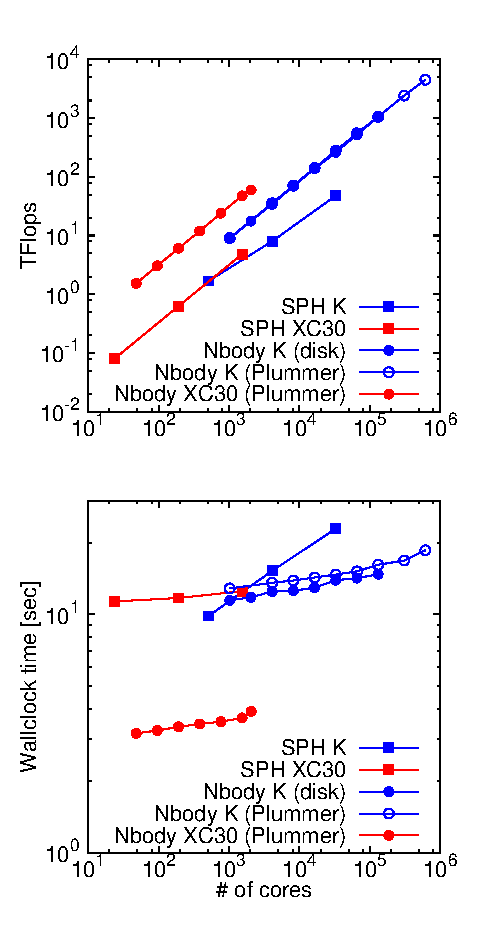
\includegraphics[width=8cm]{Flops_and_Wallclock.eps}
  \end{center}
  \caption{Performance of two applications implemented using FDPS,
    measured on K computer and Cray XC30. Top panel: Performance
    measured by the speed of floating-point operation plotted against
    the number of cores used. Bottom panel: Wallclock time per one
    timestep. Number of particles per core is 256k for $N$-body, 
    35,000 for SPH on K computer and  45,000 for SPH  on XC30.}
  \label{fig:performance}
\end{figure}

In the case of the gravitational $N$-body simulation, the achieved
performance is 50 \% and 38 \% of the theoretical peak of the machine,
when measured with 76544 and 2064 MPI processes on K computer and
XC30, respectively.  In the case of the SPH simulation, the achieved
performance is 9.1 and 7.5\%, which is not as good as what is achieved
for gravity-only calculation.

Table   \ref{tab:wallclocktime}
shows the anatomy of the wallclock time per one timestep. For both of
the gravitational $N$-body and SPH calculations, the time spent for
domain decomposition and particle exchange is a negligible fraction of
the total wallclock time per timestep. In the case of the $N$-body
simulation, the time for the communication necessary for the
interaction calculation (LET Exchange) is also small, and the total
computing time is really dominated by the time of the interaction
calculation. This is why the very high efficiency is achieved.

In the case of SPH code, we can see that the time spent for LET
exchange is larger than the time spent for the interaction
calculation.  Currently, the LET exchange for what we call
``gather-type'' short-range interactions is rather slow, even though
the actual amount of data transferred is much smaller than that
necessary for long-range interactions.  We have isolated the reason
for this inefficiency and currently working on the solution.

\begin{table}
  \begin{center}
  \label{tab:wallclocktime}
  \begin{tabular}{lcc}
    \hline
      & $N$-body & SPH\\
    \hline
    Domain decomposition & 0.0025 & 0.0054\\
    Particle exchange & 0.23 & 0.081\\
    LET Exchange  (Density \& Derivative)& --- & 5.6\\
    Force Calculation  (Density \& Derivative)& --- & 2.7\\
    LET Exchange  (Hydro)& --- & 6.6\\
    Force Calculation  (Hydro)& --- & 1.1\\
    LET Exchange  (Gravity)& 0.90 & 0.048\\
    Force Calculation (Gravity)& 11 & 0.56\\
    Total & 12 & 16\\
    \hline
  \end{tabular}
  \caption{Wallclock time for domain decomposition, particle exchange,
    Local Essential Tree (LET) exchange and  force calculation for
    runs using 512 Nodes of K computer.
  }
  \end{center}
\end{table}


The efficiency of the applications implemented using 
FDPS is comparable or higher than  those of state-of-the-art code.
GreeM 
\cite{ishiyama:gordonbell} achieved 55\% of the theoretical peak
of K computer for the cosmological $N$-body simulation with $2 \times
10^{12}$ particles. This efficiency is higher than that we achieved,
but the number of particle per node  used is more than 10 times
larger, resulting in higher efficiency.

For SPH calculation, at present the achieve efficiency is not very
high, since the interaction calculation is not the dominant part.  As
stated earlier, current implementation of the LET exchange for
short-range interactions is rather inefficient.  After this
inefficiency is removed, the efficiency of the SPH code will become
comparable to that of the gravity-only code. 


\section{Conclusion}
\label{sec:conclusion}

In this paper, we report the performance of applications developed
using our framework for particle-based simulations, FDPS. We
have demonstrated that, by using FDPS, multiple applications achieve very
good scalability without the need for spending years of time in code
development. We believe our approach will  be quite useful
for those who want to develop high-performance application code for
particle-based simulations in many different fields. 

Not only good scalability, but also the high absolute performance can
be achieved for applications developed with FDPS, because the design
concept of FDPS to provide highly efficient implementation for the
parallelization part, such as domain decomposition, particle exchange
and exchange of information necessary to calculate interaction. It is
still necessary for application developers to provide highly optimized
functions for interaction calculation. However, compared to all the
works necessary to develop,  debug and tune large-scale parallel
applications, this part is much 
easier, in particular because development and test can be done on
single-processor machines.

We demonstrated that applications with very high performance can be
developed by using FDPS. In the case of gravitational $N$-body
problem, the achieved efficiency is around 50\% of the theoretical
peak, and for SPH 10\%. These numbers are comparable or better than the
best numbers in the literature.

Thus, we believe that it is not unfair to say that FDPS offers the
researchers and/or programmers  a new and easy way to
develop large-scale particle-based simulation programs. We believe
similar approach can be applied to other types of large-scale
simulations, such as those based on regular or irregular grids.




%FDPS, \textit{FDPS}, \textbf{FDPS}, \texttt{FDPS}
%\section{Section \secit{Section}}
%\subsection{Subsection \subsecit{Subsection}}
%\subsubsection{Subsubsection}
%\paragraph{Paragraph}
%\paragraph*{Paragraph*}
%$c_\mathrm{s}$, $c_{\mathrm{s},i}$

\section{Acknowledgments}

We thank M. Fujii for providing initial conditions of spiral
simulations, T. Ishiyama for providing his Particle Mesh code, and
Y. Maruyama for being the first user of FDPS.  We are grateful to
M. Tsubouchi for her help in managing the FDPS development team. This
research used computational resources of the K computer provided by
the RIKEN Advanced Institute for Computational Science through the
HPCI System Research project (Project ID:ra000008).

\bibliographystyle{abbrv}
%\bibliography{sc15_fdps}
\bibliography{gb_sc15}

\end{document}

% LocalWords:  FDPS Masaki Iwasawa RIKEN Minatojima minami machi Chuo ku Hyogo
% LocalWords:  Ataru Tanikawa Natsuki Hosono Keigo Nitadori Takayuki Muranushi
% LocalWords:  Junichiro Makino parallelization scalability meshfree multi SIMD
% LocalWords:  Github GreeM SPH APIs du dt sc fdps Fujii Ishiyama Maruyama HPCI
% LocalWords:  Tsubouchi ra ACM XC HPC parallelized analytics TMC Xeon Haswell
% LocalWords:  interprocessor Fortran HPF vectorizing parallelize DSL MPI Bcast
% LocalWords:  OpenMP runtime complicacy subdomains substeps substep timestep
% LocalWords:  multithreading functionalities multisection octree subsamples ip
% LocalWords:  superparticles Alltoall Alltoallv GPGPUs interparticle API CPUs
% LocalWords:  GPUs CUDA OpenCL GPU CfCA SPARC VIIIfx Gflops Multipole treewalk
% LocalWords:  quadrupole Balsara impactor proto lcc TPJ struct CalcGrav const
% LocalWords:  Nbody ni jp nj vec pos ep eps ai xj dr mj dri sqrt acc epj xy zm
% LocalWords:  yi zi ay az bcl bch yj zj dx dy ri rsqrta mri nmsub noinline po
% LocalWords:  xibuf veps epjbuf FMA intrinsics wallclock gb
